\documentclass[12pt, a4paper]{article}
\usepackage{../notesheets}

%%%%%%%%%%%%%%%%%%%%%%%%%%%%%%%%%%%%%%%%%%%%%%%%%%
\author{Math 1210}
\title{Trig Identity Homework}
\date{}

\begin{document}
\maketitle
\nameline
%%%%%%%%%%%%%%%%%%%%%%%%%%%%%%%%%%%%%%%%%%%%%%%%%%
\section{Useful Trig Identities}
\begin{thrm}[Fundamental Trig Identities]
  Given any numbers \(x,y\), we have the following equalities
  \begin{enumerate}
  \item \(\sin^2 (x) + \cos^2 (y) = 1 \) \hspace{2.4in} \text(The Pythagorean identity)
  \item \(\sin(x+y) = \sin(x)\cos(y) + \sin(y)\cos(x)\) \hspace{1in}  (The sine
    sum formula)
  \item \(\cos(x+y) = \cos(x)\cos(y) - \sin(x)\sin(y)\)  \hspace{1in} (The cosine
    sum formula)
  \end{enumerate}
\end{thrm}
\vspace{-0.75in}
You must \textbf{memorize these identities} for this class. They will
show up many times throughout the semester, including on exams!
\begin{thrm}[Derived Trig Identities]
  Given any numbers \(x,y\), we have the following equalities
  \begin{enumerate}
  \item \(\tan^2(x)+1 = \sec^2(x)\)
  \item \(\cot^2(x)+1 = \csc^2(x)\)
  \item \(\sin(x-y) = \sin(x)\cos(y)-\sin(y)\cos(x)\)
  \item \(\cos(x-y) = \cos(x)\cos(y)+\sin(x)\sin(y)\)
  \item \(\sin(2x) = 2\sin(x)\cos(x)\)
  \item \(\cos(2x) = \cos^2(x)-\sin^2(x)\)
  \item \(\sin^2(x) = \frac{1}{2}(1-\cos(2x))\)
  \item \(\cos^2(x) = \frac{1}{2}(1+\cos(2x))\)
  \end{enumerate}
\end{thrm}
\vspace{-1in}
\begin{ex}
  To warm up with trig functions, find \textbf{all} values of \(\theta\) such that \(\sin^2 \theta
  = \sin \theta\). You do not need to use any trig identities, but
  consider solving \(x^2=x\) first.
\end{ex}
\pagebreak
\section{Pythagorean Identity}
\begin{ex}
Recall from notesheet 12.2 that, if a point \(P\) is on the unit
circle and forms an angle \(\theta\) with the \(x\)-axis, then, in
coordinates, \(P = (\cos \theta, \sin \theta)\). Thus, we have the
following picture:\\
\begin{minipage}{0.6\linewidth}
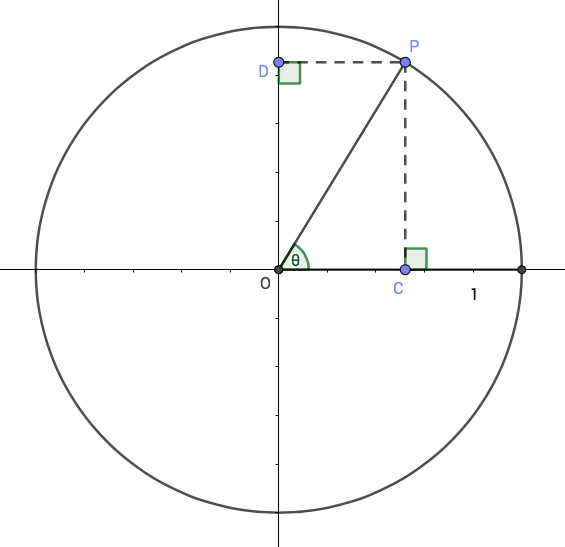
\includegraphics[scale=0.5]{images/unit-circle-with-emphasis}  
\end{minipage}
\begin{minipage}{0.4\linewidth}
  \textbf{(a) Fill in the following values in terms of \(\theta\)}
  \begin{itemize}
  \item The length of \(OC = \)
  \item The length of \(PC = \)
  \item (Does not depend on \(\theta\)). The length of \(OP = \)
  \end{itemize}
\end{minipage}
Notice that \(OCP\) forms a \emph{right triangle}. Thus, we can use
The Pythaogrean Theorem on the triangle \(OCP\).\\
\textbf{(b) Fill in the Pythagorean theorem in terms of the right
  triangle OCP to get the Pythagorean identity from Theorem 1.}
\end{ex}
\begin{ex}
  Show that \(\cot(x)+\tan(x) = \sec(x)\csc(x)\) using the definitions
  of \(\tan\) and \(\cot\), as well as the Pythagorean identity.
  \begin{enumerate}
  \item Start with \(\cot(x) + \tan(x)\) and substitute \(\tan(x) =
    \frac{\sin(x)}{\cos(x)}\). Also do the 
    likewise substitution for \(\cot(x)\).
    \vspace{1in}
  \item Find a common denominator for the sum of fractions and combine
    them.
    \vspace{1in}
  \item Simplify the numerator using the Pythagorean identity.
    \vspace{1in}
  \item Rewrite your fraction as a product of two fractions.
    \vspace{1in}
  \item Rewrite your expression using the definition of \(\sec(x)\)
    and \(\csc(x)\).
  \end{enumerate}
\end{ex}
\vspace{-1in}
\begin{ex}
  Verify \(\cot^2(x)+1 = \csc^2(x)\). Hint: Divide the Pythagorean
  identity by something.
\end{ex}
\section{Sum Identities}
\begin{ex}
  Using the fact \(\sin(x+y) = \sin(x)\cos(y)+\sin(y)\cos(x)\), verify
  \(\sin(2x) = 2 \sin(x)\cos(x)\) by setting \(x = y\).
\end{ex}
\begin{ex}
  Using any of the listed trig identities on the first page, compute
  \(\sin\left( -\frac{3 \pi}{8} \right)\)
\end{ex}
\begin{ex}
  Use the sine sum formula to prove \(\sin\left(x+\frac{\pi}{2}\right) = \cos(x)\).
\end{ex}
\section{Derivatives of Trig Identities}
Recall the definition of the derivative:
\begin{defi}
  Given a function \(f(x)\), we say its derivative \(f'(x)\) is given
  by \[
    f'(x) = \lim_{h \to 0} \frac{f(x+h)-f(x)}{h} \ \ \text{ provided
      the limit exists.}
  \]
\end{defi}
\vspace{-0.75in}
Another useful fact that we will see later is the following
\begin{thrm}[Useful fact about sine]
  \(\lim_{h \to 0} \frac{\sin(h)}{h} = 1 \implies \lim_{h \to 0}
  \frac{\cos(h)-1}{h} = 0\)
\end{thrm}
\vspace{-0.75in}
\begin{ex}
  Find the derivative of \(f(x) = \sin(x)\).
  \begin{enumerate}
  \item Do the substitution \(f(x) = \sin(x)\) into the difference
    quotient.
    \vspace{0.75in}
  \item Use a trig identity to expand \(\sin(x+h)\).
    \vspace{0.75in}
  \item Distribute the \(\lim_{h \to 0}\) term across the plus sign
    and pull any terms that depend only on \(x\) outside the limit.
    \vspace{0.75in}
  \item Using the ``Useful fact about sine'' above, evaluate the limits.
  \end{enumerate}
\end{ex}
\vspace{-1in}
\begin{ex}
  Draw a graph of \(f(x) = \sin(x)\), including at least
  \([-\pi,2\pi]\) in your \(x\)-axis. Draw the tangent line through
  the point
  \(\left(\frac{\pi}{2},\sin \frac{\pi}{2}\right)\) and also the
  tangent line through the point \(\left( \pi, \sin \pi
  \right)\). What are the slopes of these tangent lines?
\end{ex}
\begin{ex}
  Draw a graph of \(g(x) = \cos(x)\), including at least
  \([-\pi,2\pi]\) in your \(x\)-axis. Draw the tangent line through
  the point \((0, \cos(0))\) and also the tangent line through the
  point \(\left( \frac{\pi}{2}, \cos \frac{\pi}{2} \right)\). What are
  the slopes of these tangent lines?
\end{ex}
\begin{ex}
  Let \(f(x) = \sin x\) and \(g(x) = \cos x\) as above.
  \begin{enumerate}
  \item   Can you use a
  symmetry argument to see why \(f'\left(x+\frac{\pi}{2}\right) = g'(x)\)? 
  \item Simplify \(f'\left(x+\frac{\pi}{2}\right)\) to find \(g'(x)\).
  \end{enumerate}
\end{ex}
\begin{ex}
  Using what you learned above, give at least \(3\) examples of a
  function \(y(x)\) such that \[
    y(x)+y''(x) = 0
  \]
\end{ex}
%%%%%%%%%%%%%%%%%%%%%%%%%%%%%%%%%%%%%%%%%%%%%%%%%% 
\end{document}
